% !TEX root=../index.tex

\chapter{Panoramica del sistema}
\label{cap:overview}
Riproducendo la configurazione proposta in \cite{Zhu13} al soffitto del laboratorio è stato fissato un dispositivo Kinect V2 rivolto verso il pavimento.
In tale configurazione, all'ingresso di una persona nella visuale del Kinect, ne saranno ben visibili la testa e le spalle.

\section{Il Kinect}
\label{sec:sensor}
Ad onor del vero, ciò che viene comunemente chiamato \emph{sensore di profondità} (o sensore di distanza) del Kinect, è in realtà uno \emph{scanner 3D a luce strutturata}\footnote{Nonostante ciò, lo si continuerà a chiamare \emph{sensore di profondità}, leggermente inesatto, ma decisamente più breve ed intuitivo}.
\begin{wrapfigure}{r}{}
    \begin{center}
        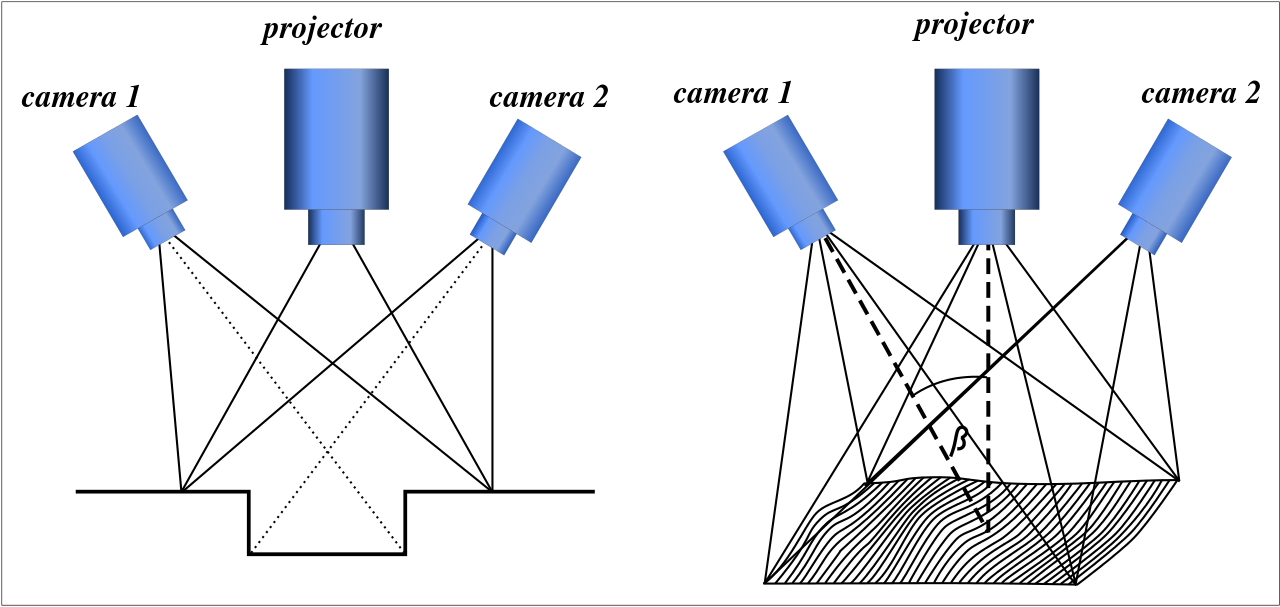
\includegraphics[width=8cm]{img/3d-structured-light-scanner.png}
    \end{center}
    \label{fig:structured_light_scanner}
    \caption{Schematizzazione di uno scanner 3D a luce strutturata.}
\end{wrapfigure}
Un sorgente di raggi infrarossi proietta una serie di pattern codificati. La deformazione indotta dalle superfici degli oggetti interessati viene acquisita da una o più telecamere ed utilizzata per il calcolo delle coordinate tridimensionali.

Il risultato di un sensore di questo tipo è un insieme di triplette $(x,y,z)$, organizzate in una \emph{immagine di profontità}, una struttura dati che è molto simile ad una semplice immagine in scala dei grigi, dove il valore di ogni pixel rappresenta la misura in millimetri della distanza della superficie dal sensore.
La forte somiglianza con le immagini in scala dei grigi è supportata dal fatto che ogni pixel è codificato utilizzando 16bit.

La massima affidabilità del sensore del Kinect si ha per distanza comprese tra $50cm$ e $4,5m$.
Il dispositivo è montato al soffitto a $2,8m$ da terra e ha un campo visivo di $70^{\circ} \times 60^{\circ}$, il quale, all'altezza del pavimento, determina un'area di cattura di circa $4m \times 5m$.

La dimensione di ogni immagine di profondità è di $512 \times 424$ pixel. Nativamente non vengono codificate in alcun modo particolare, sono delle semplici matrici di interi.
Il Kinect V2 è in grado di catturarne fino a 30 al secondo. Utilizzando un apposito software di registrazione è stato possibile mettere insieme dei video di profondità a 30 fps.

\section{Head and Shoulder Profile}
\label{sec:hasp}

\begin{wrapfigure}{l}{}
    \begin{center}
        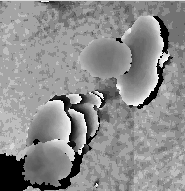
\includegraphics[width=5cm]{img/no_occlusion.png}
    \end{center}
    \caption{Due persone in un ritaglio proveniente da un frame di profondità. Il frame è stato acquisito con il Kinect V1, a differenza di quello in figura \ref{fig:spatial_feature}, acquisito con il Kinect V2.}
    \label{fig:no_occlusion}
\end{wrapfigure}

In condizioni ottimali, la figura umana ripresa dall'alto è composta solamente dalla testa e dalle spalle.
Finchè si trova quasi in corrispondenza del sensore, nella parte centrale dell'immagine di profondità, la restante parte del corpo rimane quasi del tutto nascosta. Sulla posizione delle braccia non si possono fare delle assunzioni precise.

In figura \ref{fig:no_occlusion}, la figura dell'individuo a destra corrisponde a tale descrizione, mentre dell'altro è visibile parte del corpo ed una delle due spalle è nascosta dalla testa.
Nelle zone periferiche di un frame di profondità, l'immagine è soggetta alla \emph{distorsione prospettica} così come lo è quella di qualunque telecamere RGB.

Tale distorsione costituisce un disturbo, dal momento che la figura dello stesso soggetto varia a seconda della relativa posizione nell'area di visualizzazione.
Si vedrà più avanti come affrontare tale situazione, per il momento si considerano solamente le immagini proveniente dalle zone centrali dei frame (come quella in figura \ref{fig:spatial_feature}).

Un grande vantaggio dell'utilizzo del Kinect in questa configurazione è l'\emph{assenza di occlusione}.
Infatti, rispetto ai molteplici sistemi di riconoscimento frontali, i soggetti non possono nascondersi l'uno con l'altro al sensore.

Utilizzare le immagini di profondità significa ragionare con le distanze: piuttosto che cercare di descrivere l'immagine del profilo umano in termini di forma, deve essere descritto in termini di differenze di quota rispetto all'ambiente circostante.
Alla luce di ciò, si possono identificare i seguenti criteri descrittivi:

\begin{enumerate}
    \item L'immagine di una persona è caratterizzata da uno spazio vuoto di fronte ad essa e dietro di essa. Per \emph{spazio vuoto} si intende una regione la cui distanza dal sensore è circa quella del pavimento.
    \item A sinistra della spalla sinistra ed a destra della spalla destra del profilo dall'alto di una persona, sono presenti degli spazi vuoti.
    \item Tra la testa e le spalle vi è una differenza di altezza.

\end{enumerate}

\begin{wrapfigure}{r}{}
    \begin{center}
        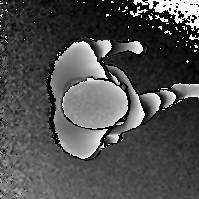
\includegraphics[width=4cm]{img/spatial_features.png}
    \end{center}
    \caption{Una persona mentre cammina}
    \label{fig:spatial_feature}
\end{wrapfigure}

Di qui in avanti, con l'acronimo \emph{HASP} (\emph{Head And Shoulder Profile}), ci si riferirà proprio al profilo della persona ripreso dall'alto che soddisfa i criteri appena elencati.

\section{Un problema di Classificazione} % (fold)
\label{sub:struttura_software}
Il software è diviso in due moduli: il modulo per il riconoscimento e il modulo di allenamento.

Nella prima fase, quella di allenamento, il relativo modulo software, a partire da un insieme di campioni classificati, genererà un insieme di regole per classificare campioni con le medesime caratteristiche. Implementa l'algoritmo Adaboost.

La seconda fase, quella di riconoscimento, lavora su dati reali: ad ogni frame acquisito tramite il sensore di profondità del Kinect si applicano le regole di classificazione generate nella fase precedente, stabilendo se nel frame è stata ripresa una persona e - in caso affermativo - la posizione di quest'ultima.
